\documentclass{article}
\usepackage{graphicx}
\usepackage{amsmath}
\usepackage{amsfonts} 
% or 
\usepackage{amssymb}

\usepackage{tikz}
\usepackage{pgfplots}
\usepgfplotslibrary{fillbetween}
\usetikzlibrary{patterns}

\pgfplotsset{compat = newest}
\usepackage{cancel}
\usepackage[margin=1in]{geometry}
\usepackage{siunitx}
\usetikzlibrary{snakes}
\usepackage{pgflibrarysnakes}
\usetikzlibrary{decorations}

\begin{document}

\section{Base Units}
There are 7 base SI base units and they are as follows:

\begin{center}
  \begin{tabular}{ | c | c | c | }
    \hline
    Name & Unit Name & Unit \\ \hline
    Time & Seconds & \si{s} \\ \hline
    Mass & Kilogram & \si{kg} \\ \hline
    Current & Ampere & \si{A} \\ \hline
    Temperature & Kelvin & \si{K} \\ \hline
    Amount of substance & Mole & \si{mol} \\ \hline
    Luminosity & Candela & \si{cd} \\
    \hline
  \end{tabular}
\end{center}

\subsection{Derived Units}
From the si base units, one can derive other units such as \si{ms^{-1}}.
We can show this with the following:
\begin{gather*}
	s = \frac{d}{t} \\
	s = \frac{\si{m}}{\si{s}} \\
	s = \si{ms^{-1}}
\end{gather*}
Another more complex example: 
\begin{gather*}
	E_k = \frac{1}{2}mv^2 \\
	E_k = \frac{1}{2}\si{kg} \left (\si{ms^{-1}} \right )^2 \\
	E_k = \frac{1}{2}\si{kgm^{2}s^{-2}} \\
	\text{We remove the constant as it adds nothing to the unit} \\
	E_k = \si{kgm^{2}s^{-2}} \\
	J = \si{kgm^{2}s^{-2}} \\
\end{gather*}

\break

\section{Uncertanty}

\subsection{Measuring devices}
The typical uncertanty of a mesuring implement such as a ruler is half a division. So, for a typical ruler it would be $0.5\si{mm}$.
However, often a ruler needs to be alighned at two ends. this means that the actual uncertatny would be $1\si{mm}$.

\subsection{Calculationg Uncertanty}
Uncertanty is calculated using the following:
\begin{equation}
	\text{uncertanty} = \frac{\text{error}}{\text{value}}
\end{equation}

\subsection{Combining Uncertanty}
When multiplying two values with a percentage uncertanty that uncertanty is summed together.
For example, if given a cube with dimensions $50 \pm 1\si{mm}$, we can calculate the uncertanty of the volume
as follows:
\begin{gather*}
	\text{Start by calculating percentage uncertanty for a single side}\\
	\frac{1}{50} = 2 \% \\
	\text{Then multiply the uncertanty by $3$ because we are doing $\left (50 \pm 1 \si{mm} \right )^3$} \\
	2\% \times 3 = 6 \% \\
\end{gather*}
\subsection{Practicle: Measuring Density with Uncertanty}

\begin{center}
  \begin{tabular}{ | c | c | c | }
    \hline
    Mass & Volume & Density \\
	\hline	
    $550.2\si{g} \pm 0.05\si{g} (\pm 0.00908\%)$ & $(49 \pm 1\si{mm}(\pm 5\%))$ & $11200 \pm 101\si{kgm^{-3}}(\pm 9.05 \%)$ \\
	& $\times (20 \pm 1 \si{mm}(\pm 2.04\%))$ & \\
	& $\times (50 \pm 1 \si{mm}(\pm 2 \%))$ & \\
	& $ = 49 \pm 4.42 \si{cm^3}(\pm 9.04 \%)$ & \\
    \hline
  \end{tabular}
\end{center}

\break

\section{Archimedes' Priciple}
Upthrust in fluid is equal to that of the fluid displaced.

\subsection{Application}
Archimedes principle can be used to predict the resultant force of an object partially or fully submerged in a liquid.

\subsubsection{Example}
Given a granite cube with dimensions of length $3\si{cm}$ submerged in \textbf{water} suspended from a newton meter, predict the value on
the newton meter.

\begin{center}
	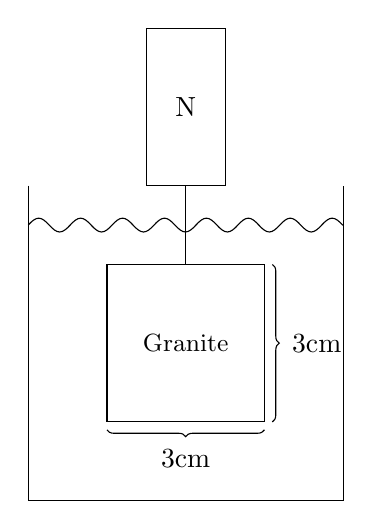
\begin{tikzpicture}
	\draw (-1,-1) rectangle (1,1);
	\draw (-0.5,2) rectangle (0.5,4);
	\draw (-2,2) -- (-2,-2) -- (2,-2) -- (2,2);
	\draw[snake=coil,segment aspect=0, line around snake=0, segment length=15.15] (-2,1.5) -- (2,1.5);
	\draw[] (0,2) -- (0,1);
	\node[] (n) at (0,3) {\si{N}};
	\node[] (m) at (0,0) {\small Granite};
	\node[label={[label distance=0.1]below:$3\si{cm}$}] (w) at (0,-1.1) {};
	\draw[snake=brace] (1,-1.1) -- (-1,-1.1);
	\draw[snake=brace] (1.1,1) -- (1.1,-1);
	\node[label={[label distance=0.1]right:$3\si{cm}$}] (w) at (1.1,0) {};
	\end{tikzpicture}
\end{cnter}

\begin{gather*}
	\text{Calculate the volume of the cube in \si{m^3}} \\
	0.03^3 = 0.000027 \si{m^3} \\
	\text{Calculate the mass of granite} \\
	0.000027 \si{m^3} \times \overbrace{2750\si{kgm^i{-3}}}^{\text{Density}} = 0.07425\si{kg} \\
	\text{Calculate the weight of granite} \\
	0.07425\si{kg} \times \overbrace{9.81\si{ms^{-2}}}^{\text{Feild Strength}} = 0.7839\si{N} \\
	\text{Volume of water displaced is the same as the volume of the cube because it is submerged}\\
	\text{Calculate the mass of water} \\
	0.000027\si{m^3} \times \overbrace{1000\si{kgm^{-3}}}^{\text{Density}} = 0.027\si{kg} \\
	\text{Calculate the upthrust} \\
	0.027\si{kg} \times \overbrace{9.81\si{ms^{-2}}}^{\text{Feild Strength}} = 0.26482\si{N} \\
	\text{Calculate the resultant force} \\
	0.72839 \si{N} - 0.26487 \si{N} = 0.464 \si{N} \\
\end{gather*}

\end{document}
